%-------------------------------------------------------------------------------
\section{Evaluation}
\label{s:eval}
%-------------------------------------------------------------------------------

This section answers the following questions:
\begin{enumerate}
    \item Does \schedbe{} isolate LC from BE workloads?
    \item Can parked processes resume correctly?
    \item How much does \schedbe{} cost?
\end{enumerate}

All the graphs in this paper run on Linux version 6.14.2, the baseline version
that our implementation builds on.

\subsection{Does \schedbe{} isolate?}

\begin{figure}[t]
    \centering
    \begin{subfigure}{\columnwidth}
        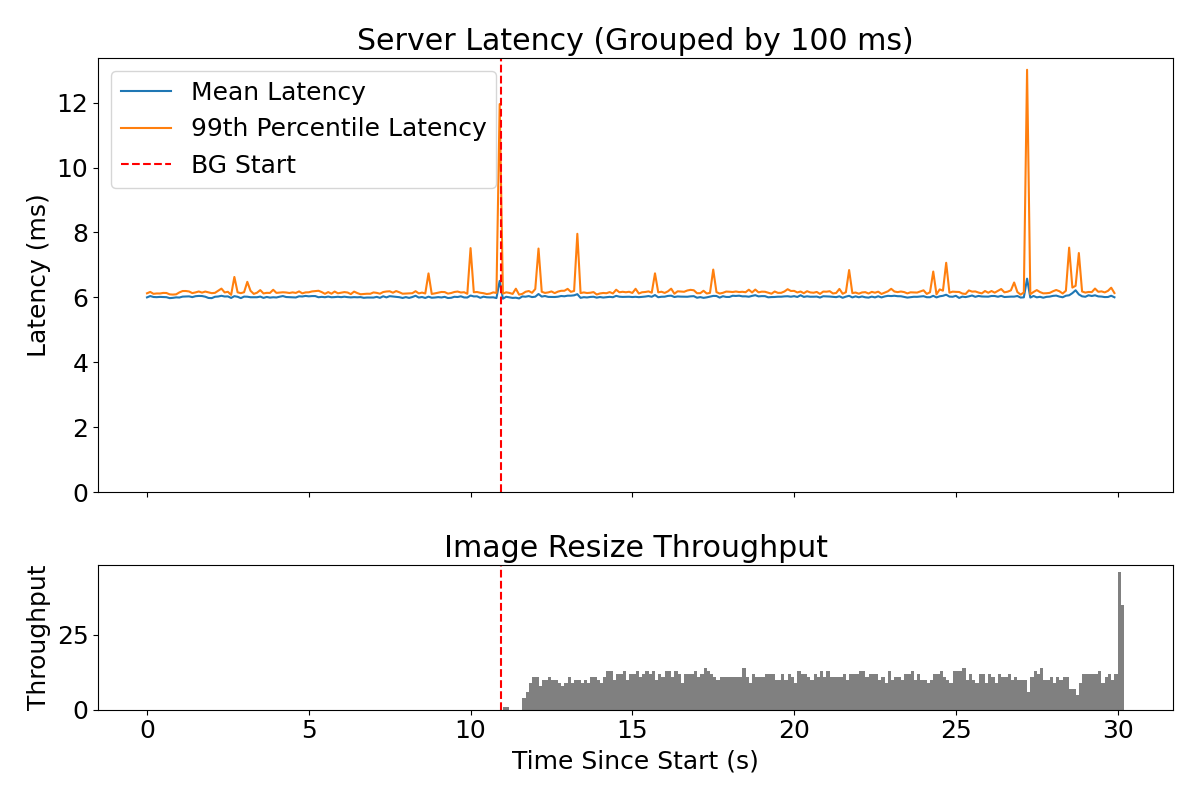
\includegraphics[width=\columnwidth]{graphs/srv-bg-schedbe-low.png}
        \caption{Low load (85\%)}\label{fig:srv-bg-schedbe-low}
        \vspace{12pt}
    \end{subfigure}
    \begin{subfigure}{\columnwidth}
        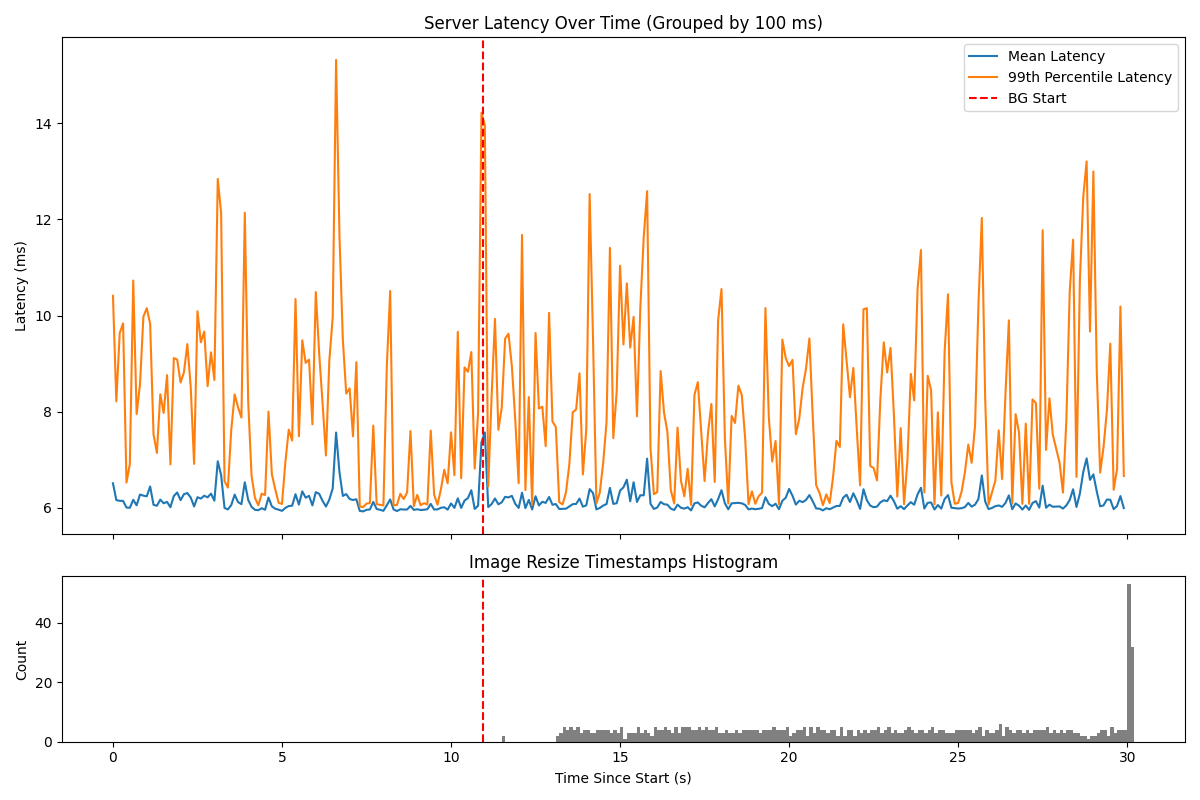
\includegraphics[width=\columnwidth]{graphs/srv-bg-schedbe-high.png}
        \caption{High load (95\%)}\label{fig:srv-bg-schedbe-high}
    \end{subfigure}
    \vspace{4pt}
    \caption{same expiriment as in \autoref{fig:srv-bg-unedited}, but with the
    BEs running in \schedbe{}}\label{fig:srv-bg-schedbe}
\end{figure}

\begin{figure}[t]
    \centering
    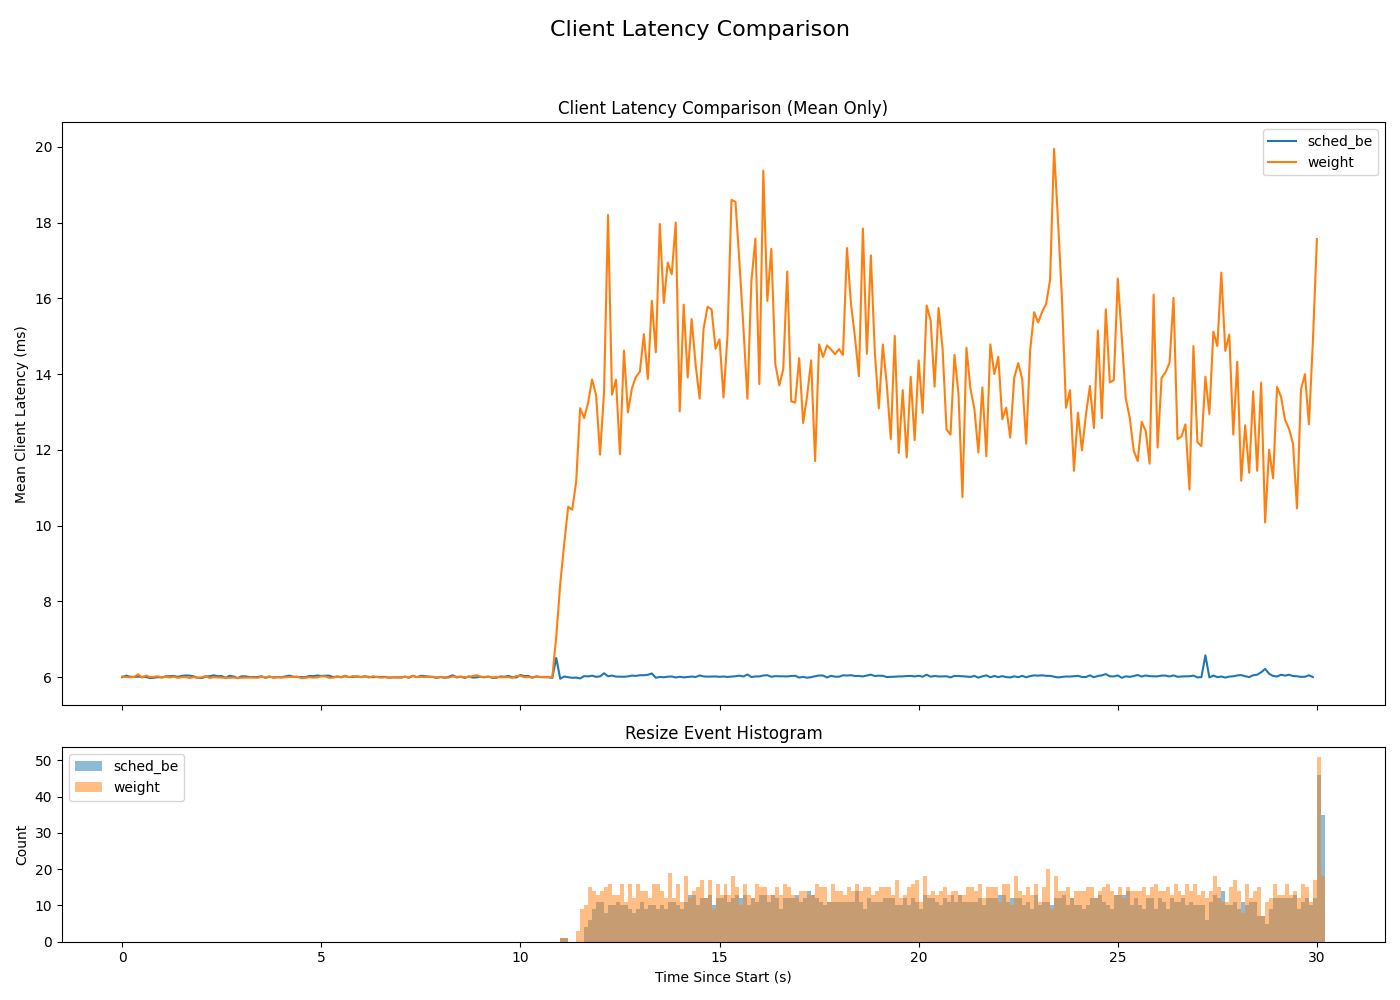
\includegraphics[width=\columnwidth]{graphs/srv-bg-cmp-unedited-schedbe.png}
    \caption{A direct comparison between the server latencies when using the
    existing \cgroups{} weights versus \schedbe{} to isolate the LC from the
    BE}\label{fig:srv-bg-cmp-unedited-schedbe}
\end{figure}

\begin{figure}[t]
    \centering
    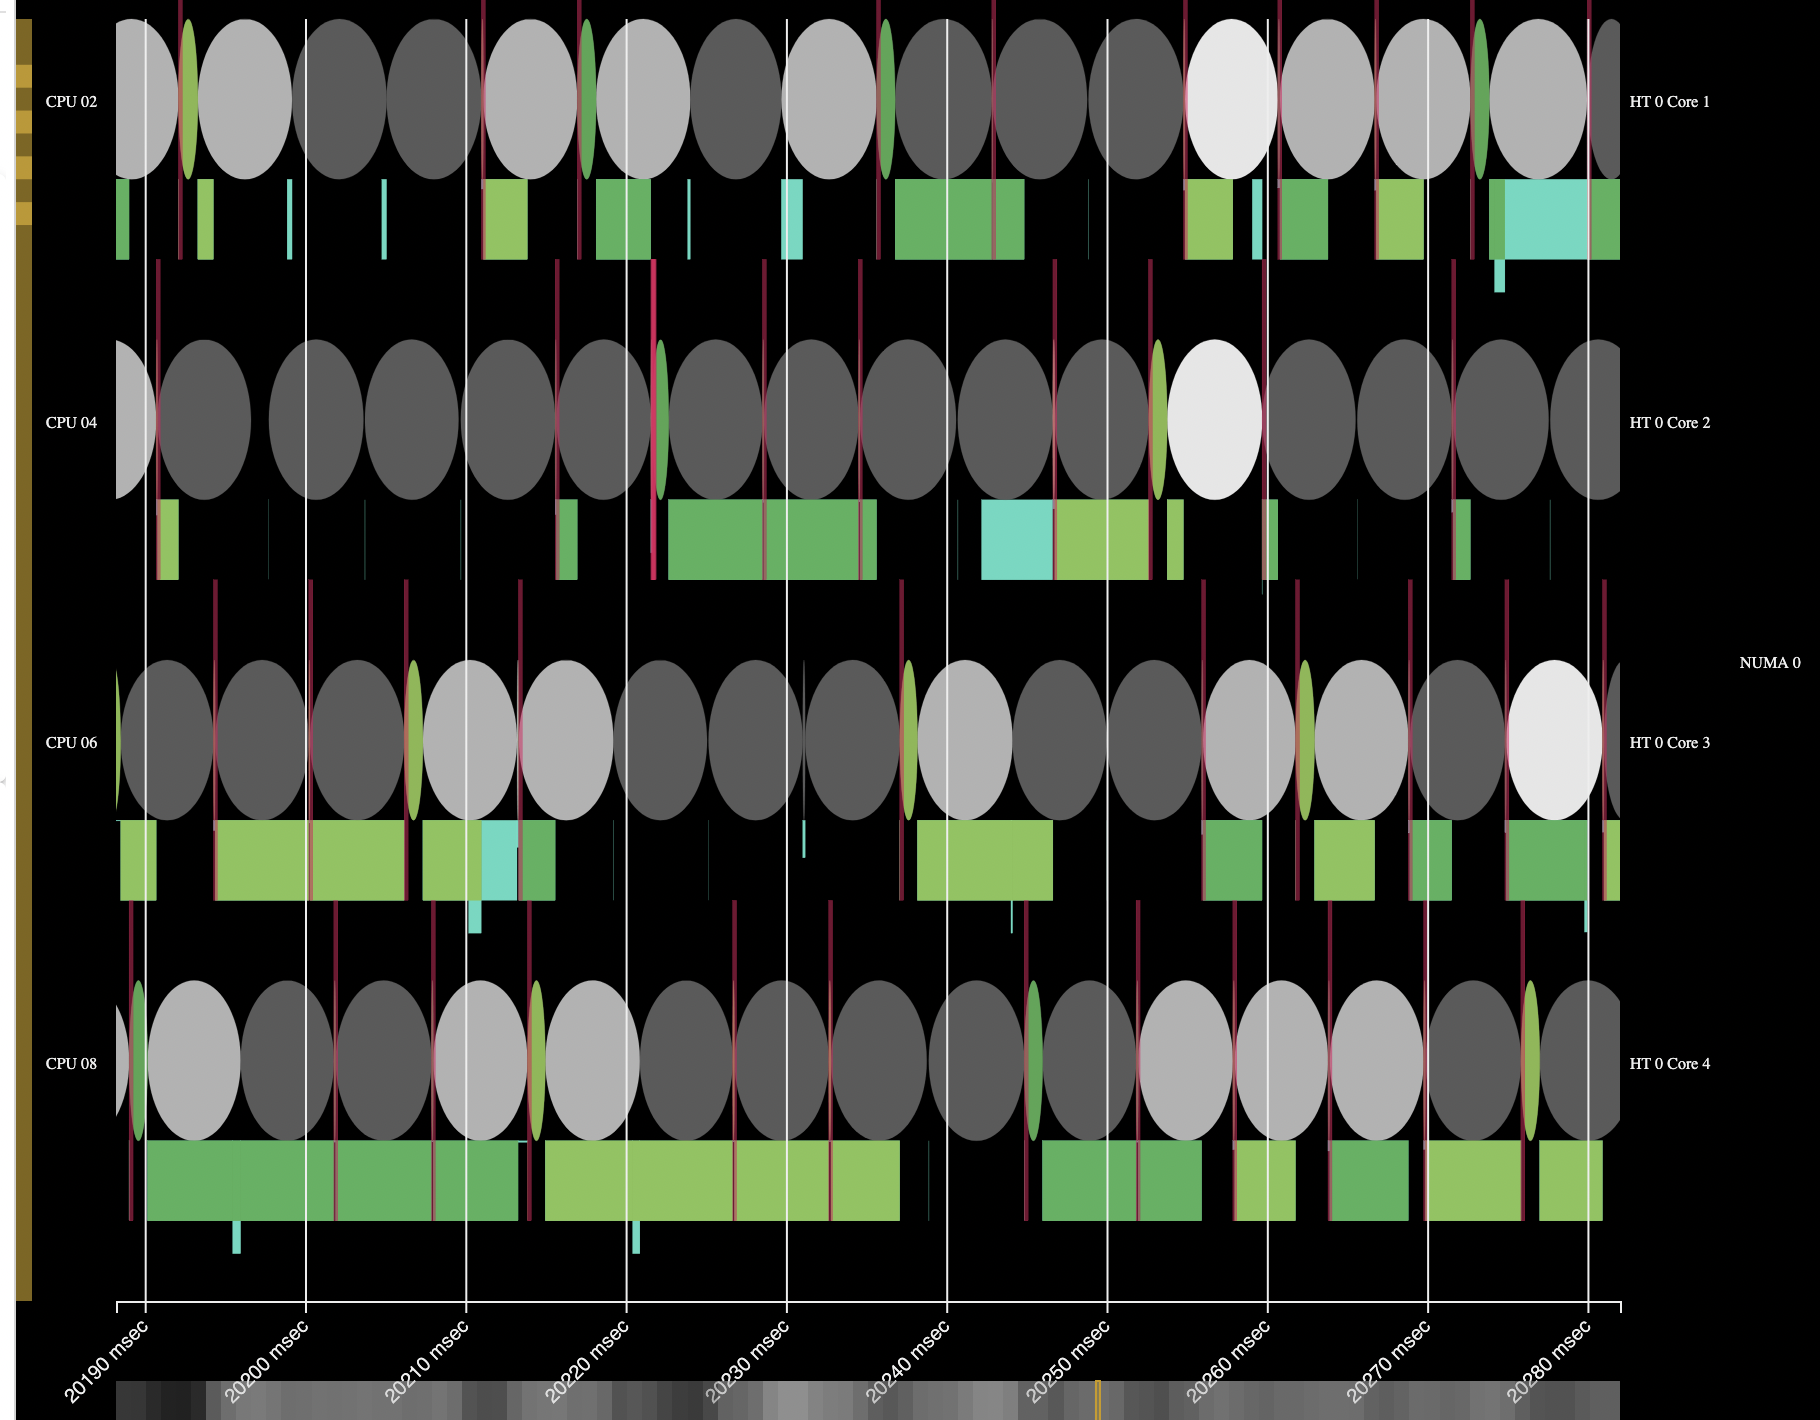
\includegraphics[width=\columnwidth]{graphs/schedviz-schedbe.png}
    \caption{BE threads only run in the gaps when there are no queued LC
    threads. The BE threads are colored in two different shades of green, the LC
    threads are the grey ones (all the threads are the same shade of grey, the
    different shades have to do with the amount of processes the visualizer has
    grouped). The red vertical lines are the scheduler initially choosing a BE
    thread, which leads to an attempt to steal a queued LC one.
    }\label{fig:schedviz-schedbe}
\end{figure}

We run the microbenchmark experiment from \autoref{fig:srv-bg-unedited} using
\schedbe{}. We can see the resulting performance in
\autoref{fig:srv-bg-schedbe}, and \autoref{fig:srv-bg-cmp-unedited-schedbe}
shows a direct comparison between the original benchmark run on \cgroups{}
weights and running it using \schedbe{}. As desired, the latency of the server
remains stable after the background tasks start. This does not mean that the
background task never runs: the lower part of each graph still shows iterations
of image resizing being done. The difference is that now the background tasks
will reliably get interrupted when the LC server has a request to process.
\autoref{fig:schedviz-schedbe} shows this happening in an outtake of a schedviz
visualization. The green BE processes run only in the gaps where there is no
queued LC process, and are immediately preempted when one wakes up, on whatever
core that may be. The vertical red lines show when the \exit{} path \schedbe{}
introduced runs, \ie{} when the core has chosen intially to run a BE process. As
we can see, this is sometimes followed by just running the BE, but often by the
core running an LC process, meaning that it succesfully found and stole a queued
and waiting LC thread.

\begin{figure}[t]
    \centering
    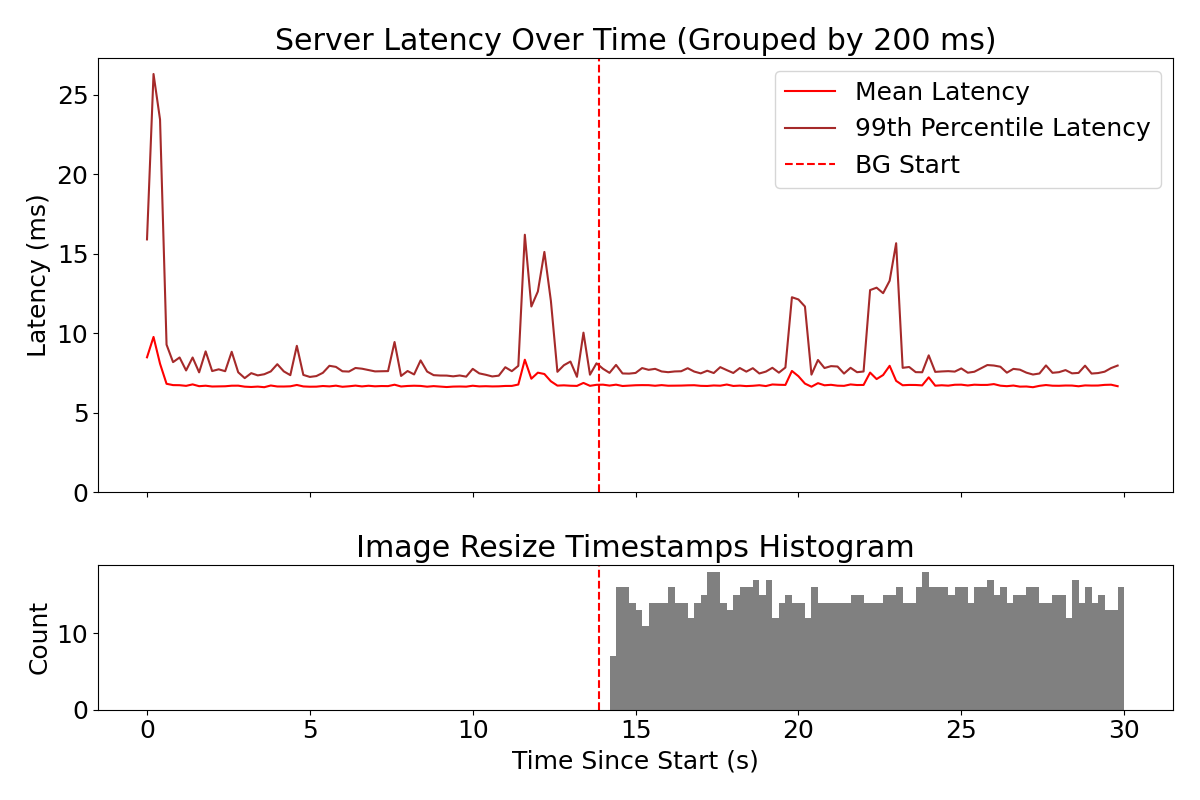
\includegraphics[width=\columnwidth]{graphs/kubernetes-schedbe.png}
    \caption{The same experiment as in \autoref{fig:kubernetes-unedited}, but
    running the BE as a \schedbe{} task}\label{fig:kubernetes-schedbe}
\end{figure}

We also run the Kubernetes application from \autoref{fig:kubernetes-unedited}
using \schedbe{}. The results are in \autoref{fig:kubernetes-schedbe}. We can
see that again the latency profile of the LC web application looks largely the
same before and after starting the image resize job. It is not entirely without
spikes, but the spikes come from interference with Python runtimes and
Kubernetes controllers, and are the same before and after starting the BE tasks.
Importantly, the baseline median latency of the LC web application stays stable
at around 7.4ms after starting the the BE image resizing. 

\subsection{Can parked processes resume correctly?}\label{ss:eval:parking}


\begin{figure}[t]
    \centering
    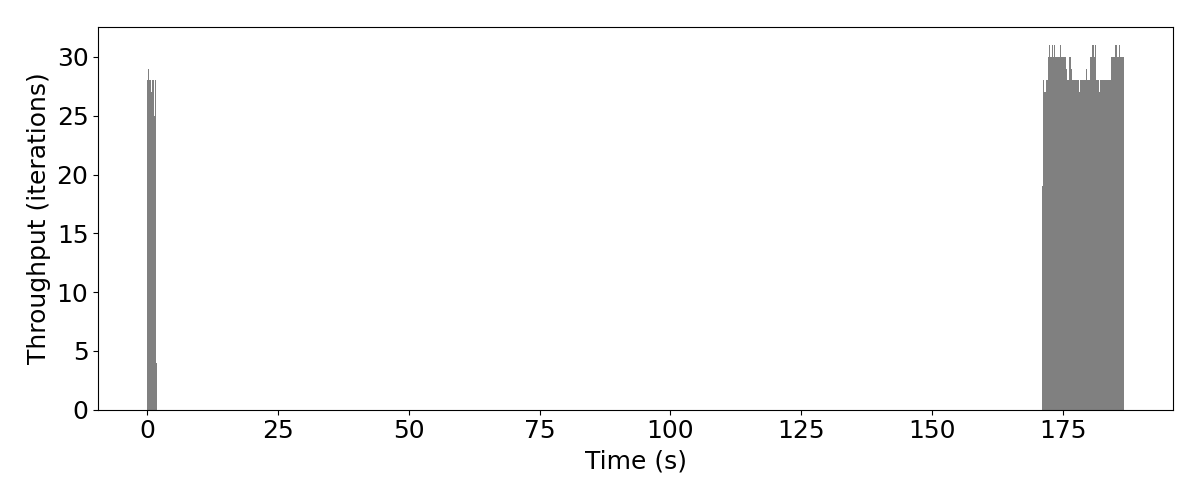
\includegraphics[width=\columnwidth]{graphs/parked-kubernetes.png}
    \caption{A \beclass{} process in a Kubernetes pod, parked while the
    antagonist runs and then resuming}\label{fig:parked-kubernetes}
\end{figure}

We investigate parking by running a BE Kubernetes pod alongside an antagonist,
and find that even after being parked for multiple minutes in the middle of
processing a request, the BE job is able to resume and return the final result
to the client. \autoref{fig:parked-kubernetes} shows the throughput over time of
an image resize job running in a BE container running as \schedbe{}. A couple
seconds after sending a request to the image resize pod, we start an entirely
CPU-bound antagonist on the same set of cores as the BE is running. We can see
that the image resize job is completely paused for about two and a half minutes,
until the antagonist is done running. The job then continues and completes. The
client connection did not experience any issues, even when setting the TCP
keepalive timeout to expire within duration the BE spent being parked.



\subsection{Cost of \schedbe{}}

The cost of \schedbe{} is can be broken down into the three checks that make up
the priority enforcement:

\begin{enumerate}
    \item \local{} adds a small amount of compute overhead on each scheduling
    decision, and removes some as well because it gets rid of the eligiblity
    check. This is a small amount of code we do not expect to impact latency
    \item \entry{} adds no new latency to Linux, which already implements
    \entry{} for \schedidle{}
    \item \exit{} adds overheads in two places: one is the cross-core check that
    each happens at each class boundary crossing, and the other is the overhead
    of the migration should it decide to steal a \schednormal{} process
\end{enumerate}

We measure the amount of time that the \exit{} check takes, and look at how
often it happens as well as how often it chooses to steal in the Kubernetes
experiment. The overhead of stealing the LC job is known, and is a complicated
function of the CPU architecture and which cores it is moving between (\eg{} how
much memory hierarchy do the two cores share).

\hmng{todo the measurements}


\subsection{Existing approaches}\label{ss:eval:existing}

To show the benefits of \schedbe{}, we compare with existing alternatives to
\cgroups{} within Linux.

\subsubsection{Realtime scheduling}

As we discussed in \autoref{s:design}, Linux enforces the strict priority
between tasks in different scheduling classes. 

This points to a possible alternative to using \cgroups{}: run LC in the real
time \rtclass{} scheduling class and BE in \normalclass{}.\footnote{The
\deadlineclass{} scheduling class is not a good fit, since it requires accurate
knowledge of a processes runtime (processing time per request) and period (when
requests come in)} \rtclass{} has two different scheduling policies:
\schedfifo{} and \schedrr{}. Both have 99 priorities between which they enforce
strict priority; within priorities \schedfifo{} enforces a global
first-in-first-out ordering based on when processes become runnable, and
\schedrr{} does round-robin scheduling.

\begin{figure}[t]
    \centering
    \begin{subfigure}[t]{\columnwidth}
        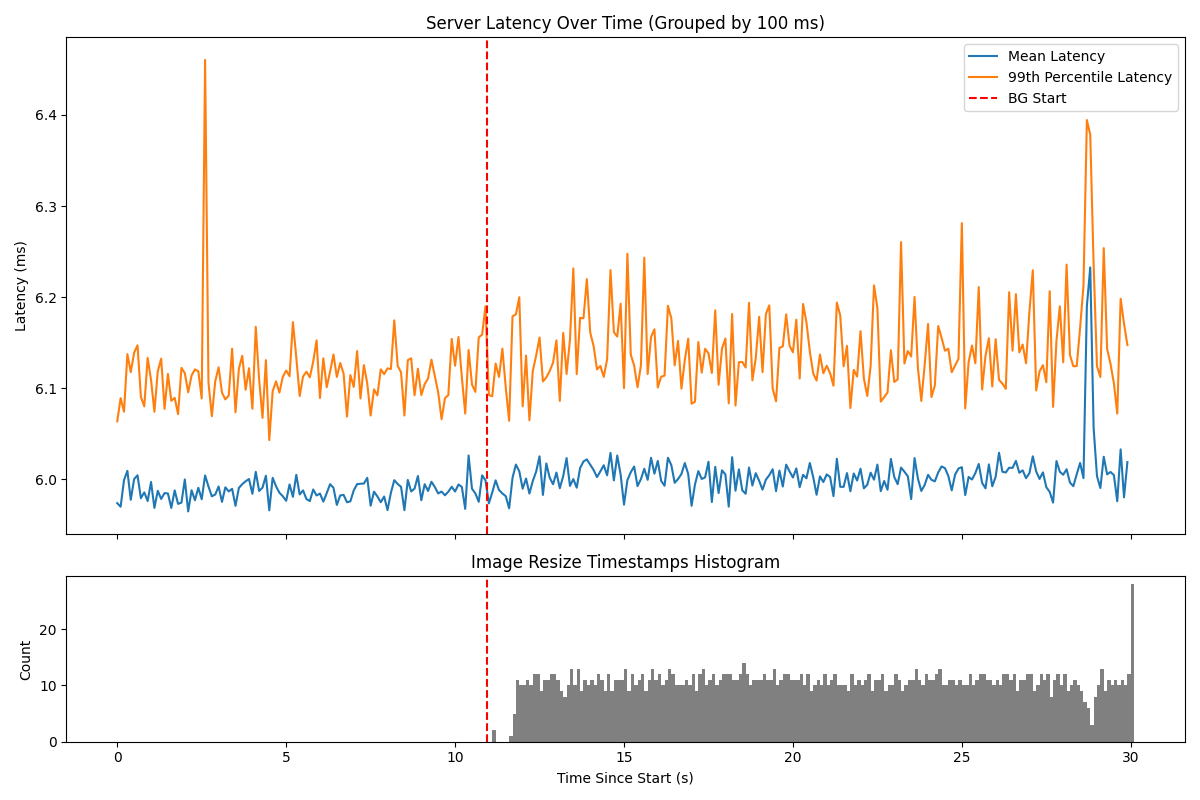
\includegraphics[width=\columnwidth]{graphs/srv-bg-rt-low.png}
        \caption{Low load}\label{fig:srv-bg-rt-low}
        \vspace{12pt}
    \end{subfigure}
    \hspace{\fill}
    \begin{subfigure}[t]{\columnwidth}
        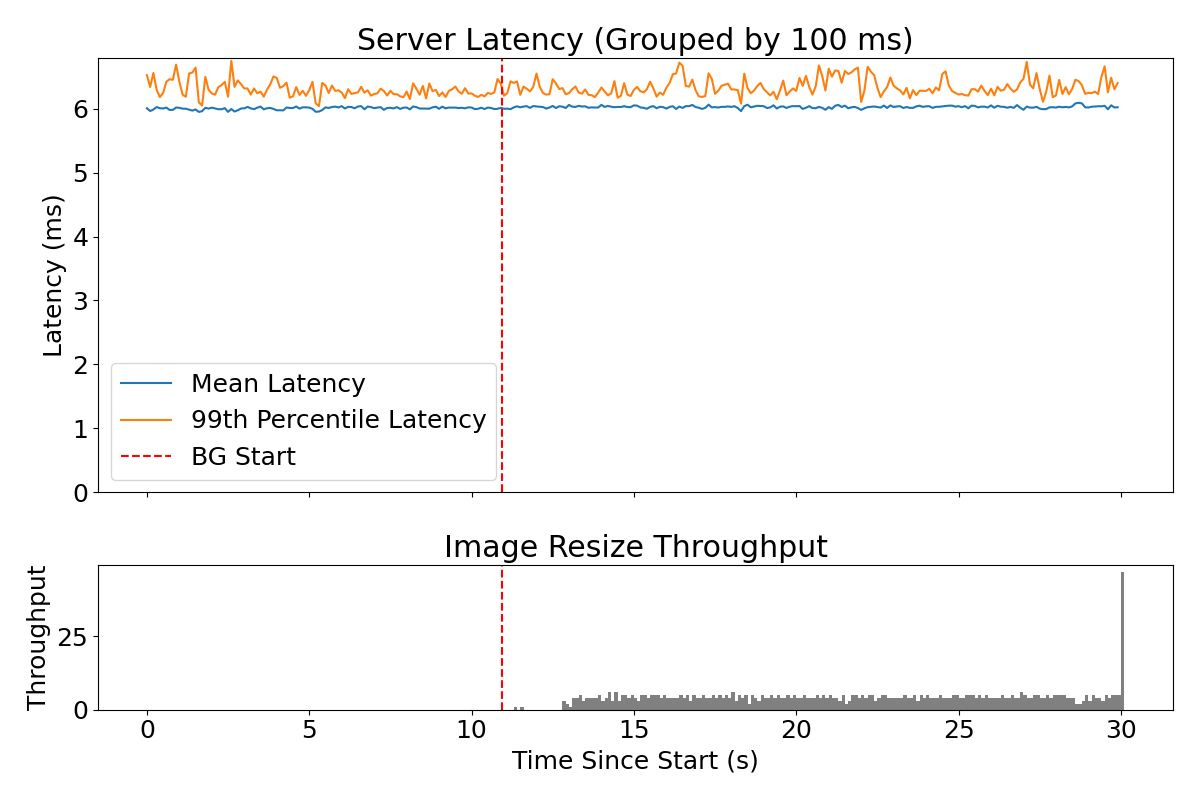
\includegraphics[width=\columnwidth]{graphs/srv-bg-rt-high.png}
        \caption{High load}\label{fig:srv-bg-rt-high}
    \end{subfigure}
    \vspace{4pt}
    \caption{Results of the same experiment as in \autoref{fig:srv-bg-unedited}
    and \autoref{fig:srv-bg-schedbe}, with LC running as a real time
    process}\label{fig:srv-bg-rt}
\end{figure}

\autoref{fig:srv-bg-rt} shows the result of running the same microbenchmark from
\autoref{fig:srv-bg-unedited} with the LC server in the \rtclass{} scheduling
class. We can see that \rtclass{} is isolated from \normalclass{} well.

However, running LC in \rtclass{} is an untenable solution because of
\rtclass{}'s intra-priority schedulers. \schedfifo{} uses run-to-completion
scheduling, which is known to have a failure mode of head-of-line (HoL) blocking
under varied request processing times, where long-running requests monopolize
the CPU while short requests wait in the queue. \schedrr{} addresses this
concern by running a round-robin scheduler that will ensure Processor Sharing
within priorities. However, \schedrr{} has no way way of enforcing unequal
splits, every process just gets the same scheduling quantum and then gets put at
the end of that priority's queue. Unequal splits is precisely what weights are
good at, and why they are used for LC services today.


\begin{figure}[t]
    \centering
    \begin{subfigure}[t]{\columnwidth}
        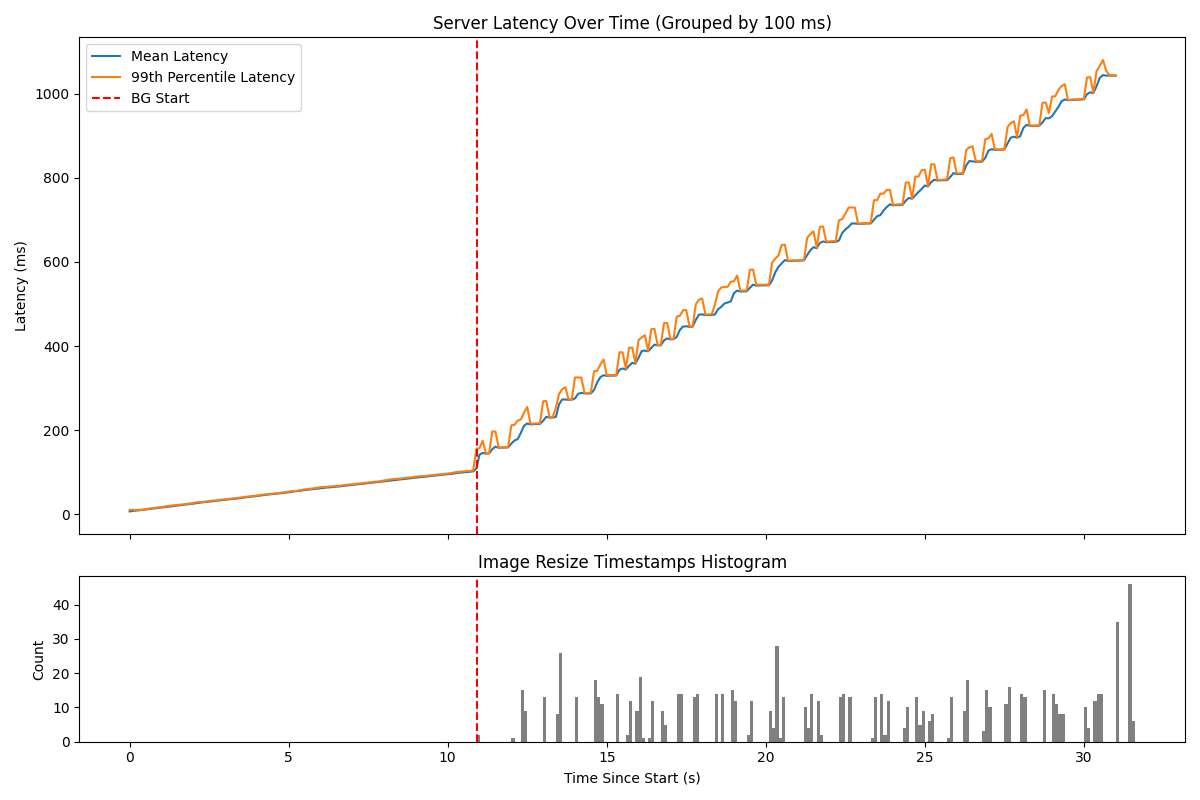
\includegraphics[width=\columnwidth]{graphs/overload-rt.png}
        \caption{LC in real time, throttling}\label{fig:overload-rt}
        \vspace{12pt}
    \end{subfigure}
    \hspace{\fill}
    \begin{subfigure}[t]{\columnwidth}
        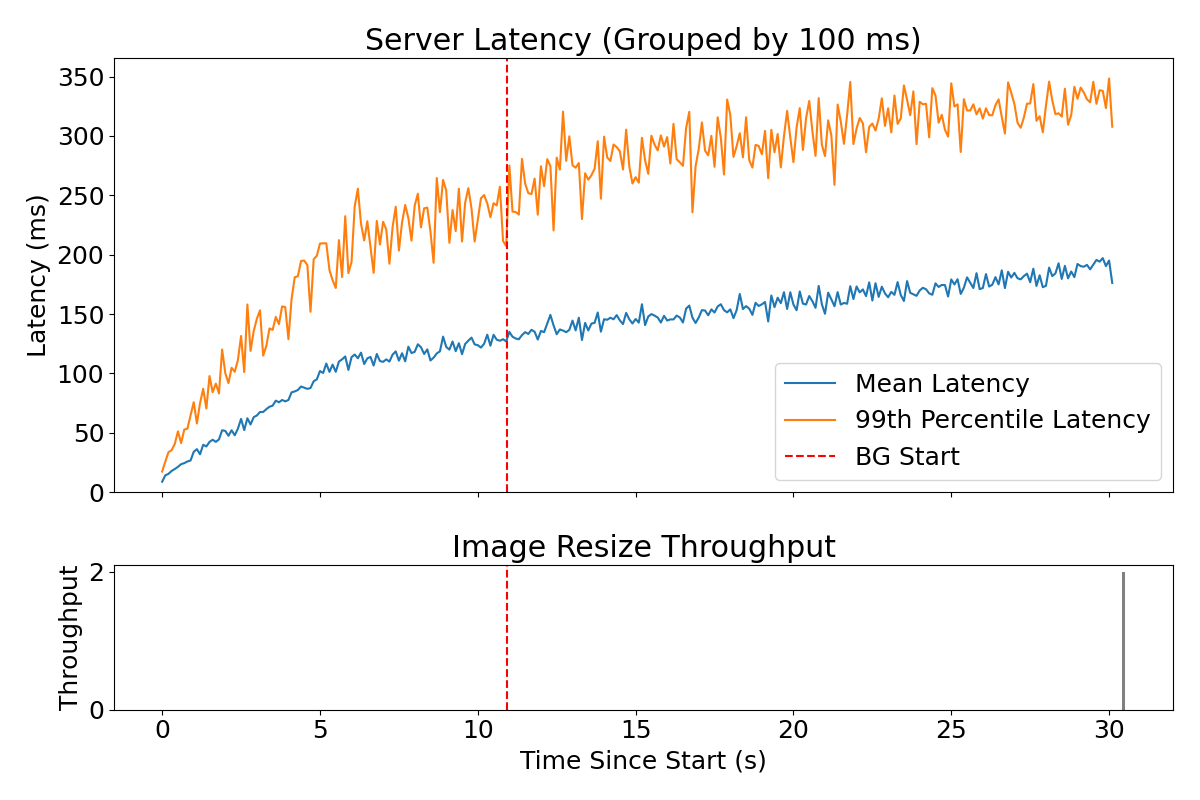
\includegraphics[width=\columnwidth]{graphs/overload-schedbe.png}
        \caption{BE in \schedbe{}, no throttling}\label{fig:overload-schedbe}
    \end{subfigure}
    \vspace{4pt}
    \caption{throttling the LC server under extremely high utilization, versus
    letting it park the BE userspace processes}
\end{figure}

In addition, under high utilization of real time processes, Linux does not park
the lower class processes or do something equivalent, but instead throttles the
\rtclass{} LC processes~\cite{lkml-deadline-srv}. We can see this happen when
we run the same microbenchmark experiment at a much higher baseline utilization
($\sim$ 100\%). The results are in \autoref{fig:overload-rt}. We see spikes
begin to appear after starting the BE task, as the \rtclass{} server gets
throttled in favor of running the BE tasks; we see parallel spikes in the BE's
throughpu in the bottom graph. Notice also the increase of the slope of response
times after starting the background tasks.

By comparison, \autoref{fig:overload-schedbe} shows what happens if, in that
same experiment, \schedbe{} allows the BE userspace process to be parked. Notice
that the BE does not make progress until the very end, when the server is done
processing the requests (the experiment stops the client after 30 seconds and
the server from then finishes the backlog of requests).

The takeaway is that Linux's mechanism of scheduling classes can isolate
workloads effectively, but existing scheduling classes use algorithms that are
not a good fit for modern workloads, and throttle the higher class under high
load.

\subsubsection{\schedidle}\label{ss:schedidle}

As discussed in \autoref{s:implementation}, \schedidle{} implements some but not
all of the isolation required of \beclass{}: it implements the \entry{} check,
but not the \exit{} check or strict local priorities.

\begin{figure}[t]
    \centering
    \begin{subfigure}[t]{\columnwidth}
        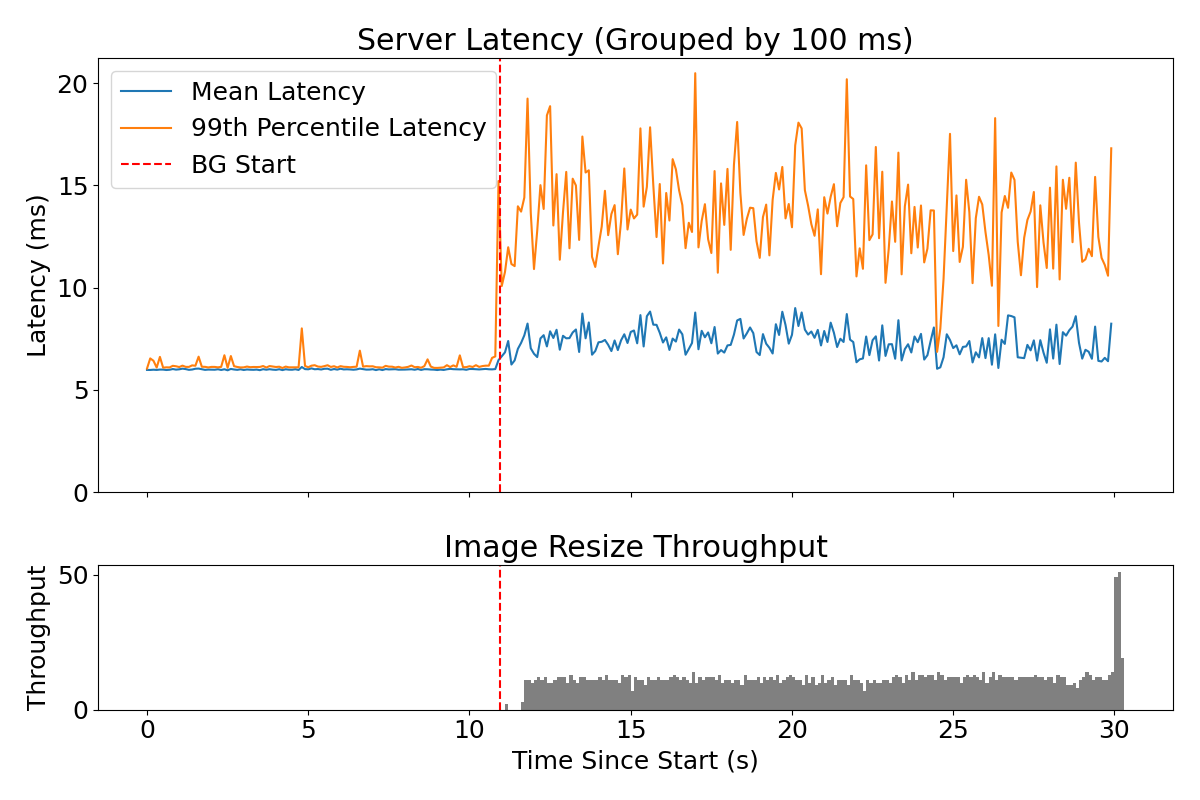
\includegraphics[width=\columnwidth]{graphs/srv-bg-idle-low.png}
        \caption{\schedidle{} in low load (85\%)}\label{fig:srv-bg-idle-low}
        \vspace{12pt}
    \end{subfigure}
    \hspace{\fill}
    \begin{subfigure}[t]{\columnwidth}
        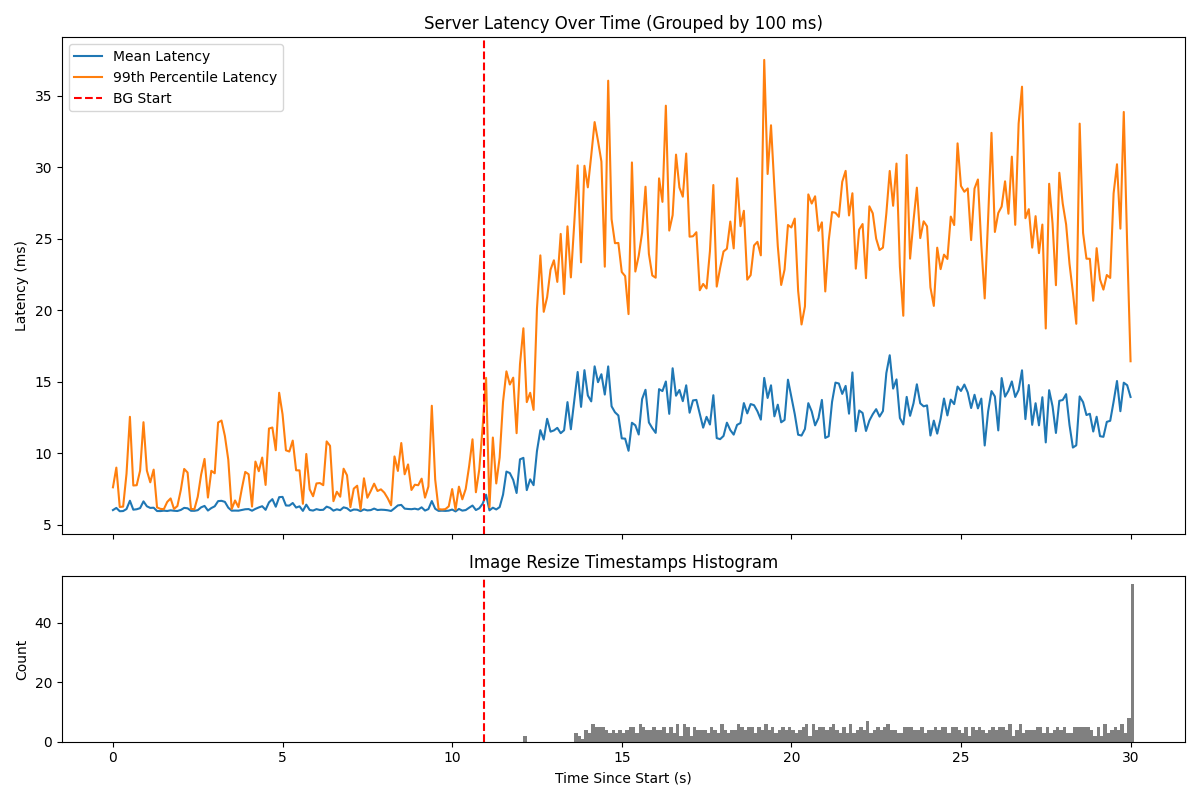
\includegraphics[width=\columnwidth]{graphs/srv-bg-idle-high.png}
        \caption{\schedidle{} in high load (95\%)}\label{fig:srv-bg-idle-high}
        \vspace{12pt}
    \end{subfigure}
    \hspace{\fill}
    \begin{subfigure}[t]{\columnwidth}
        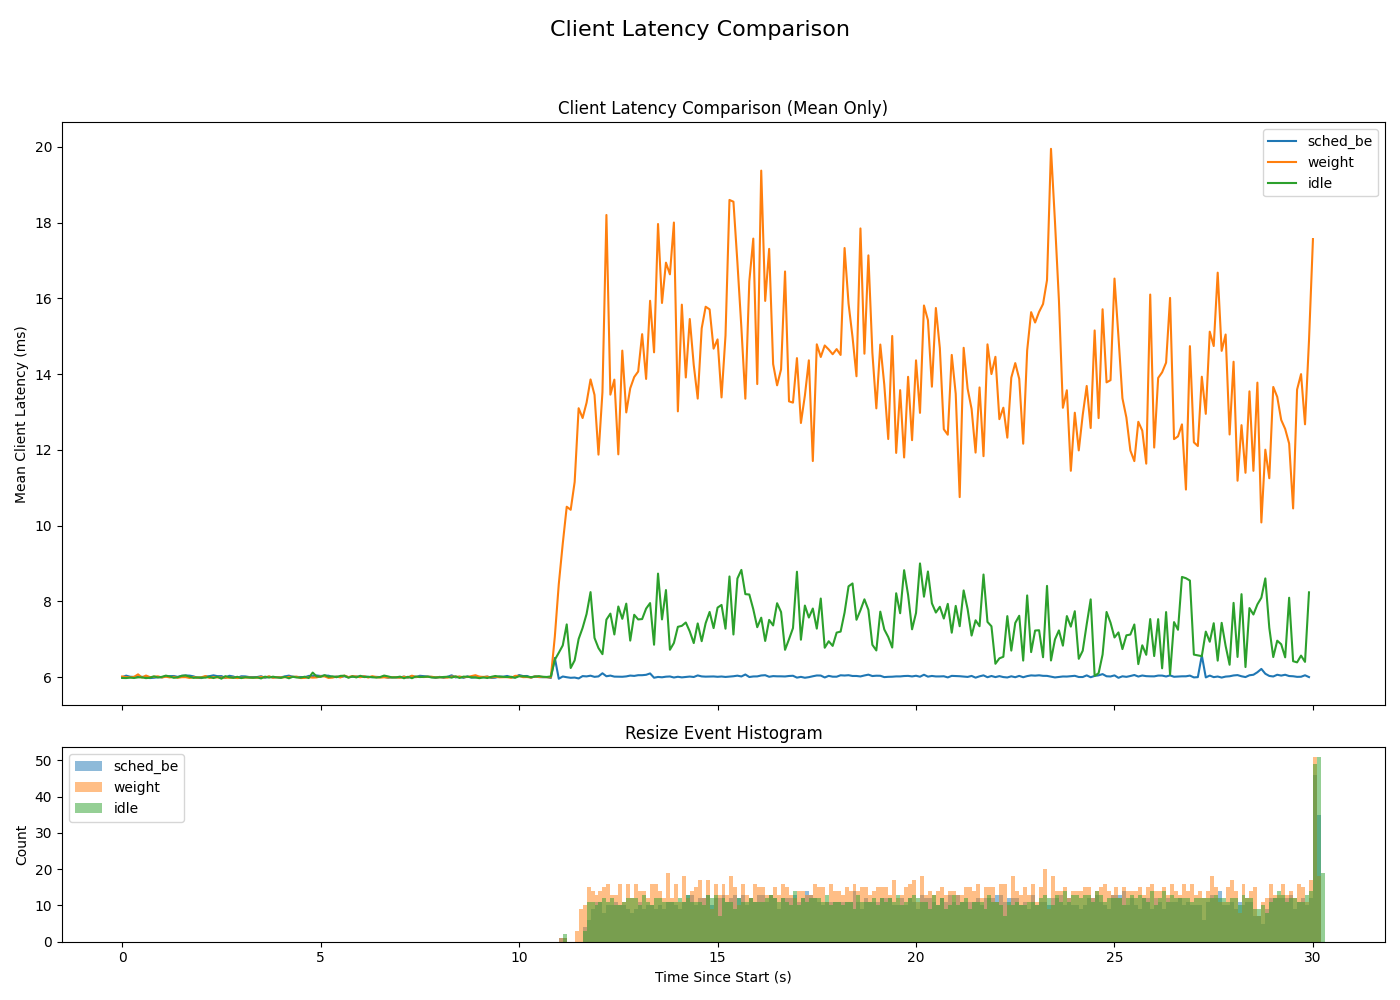
\includegraphics[width=\columnwidth]{graphs/srv-bg-cmp-all.png}
        \caption{Comparison of mean latency of the low load setting for weights,
        \schedidle{}, and \schedbe{}}\label{fig:srv-bg-cmp}
    \end{subfigure}
    \vspace{4pt}
    \caption{}\label{fig:srv-bg-idle}
\end{figure}

\begin{figure}[t]
    \centering
    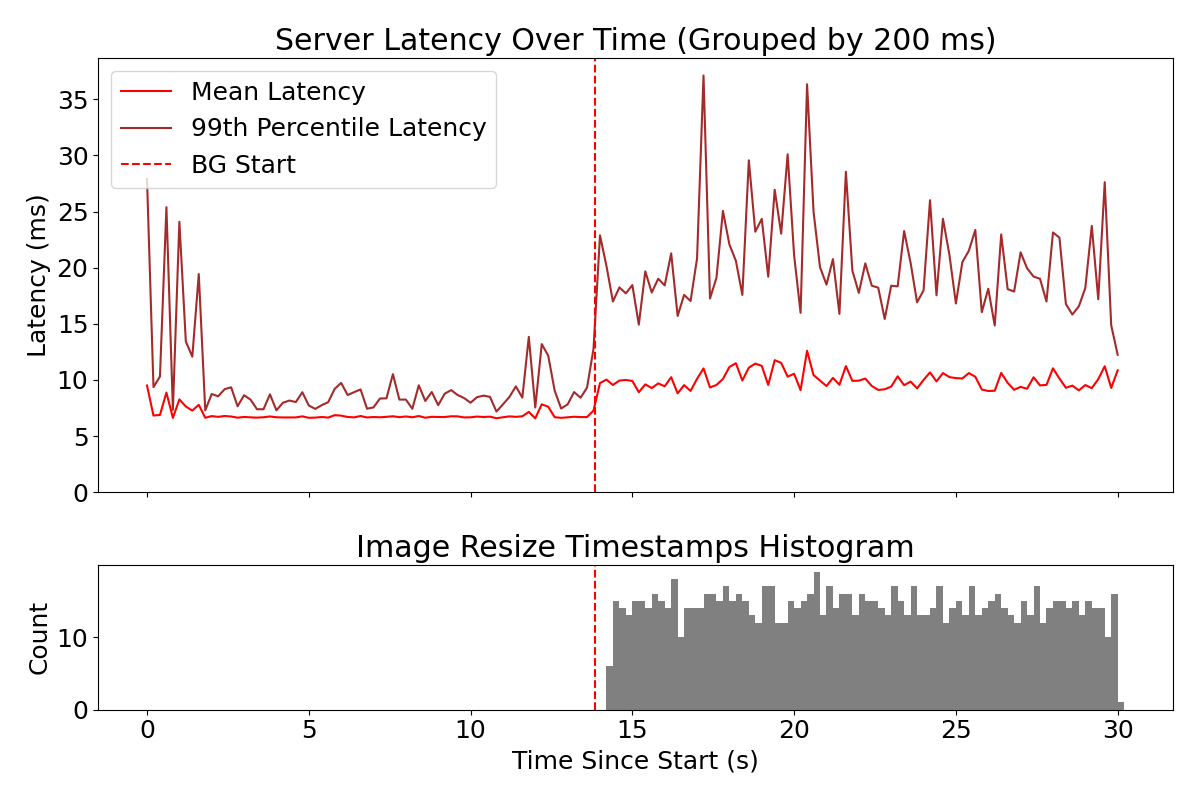
\includegraphics[width=\columnwidth]{graphs/kubernetes-idle.png}
    \caption{The same experiment as in \autoref{fig:kubernetes-unedited}, but
    running the BE as a \schedidle{} task}\label{fig:kubernetes-idle}
\end{figure}

\autoref{fig:srv-bg-idle} shows the result of running the BE jobs in the
microbenchmark in \schedidle{}, as well as a graph that compares the low load
setting of the standard \cgroups{} weight, \schedbe{}, and \schedidle{}. Average
latency still increases from $\sim$6ms to $\sim$8ms in the low load setting.
Although this increase is smaller than the original increase to $\sim$15ms using
the standard weight interface, it is still high compared to the 0ms increase
that \schedbe{} achieves. \autoref{fig:kubernetes-idle} shows similar results
for the Kubernetes experiment.